

\section{Additional Experimental Results}

We now provide further details and results
from Section~\ref{sec:exp}, which we omitted
due to space limitations from the main body.
We begin by providing further details
of the sigmoid threshold influence function
and then provide omitted details
and results for synthetic instances.

\spara{Sigmoid threshold influence function}

\begin{algorithm}
\caption{Flipping the Median via the Sigmoid Threshold Influence Function.}
\label{alg:sigmoid}
\begin{algorithmic}[1]
\Function{SigmoidGD}{$G, \alpha_0, s, k, \eta$}
    \State $\alpha \gets \alpha_0$
    \While{not converged}
        \State Let $X = I - (I - A) M$ where $A = \mathrm{Diag}(\alpha)$
        \State Solve $x^\star = \min_x \|X x - A s \|_2$
        \com{Calculate opinions}
        \State $\alpha' \gets \alpha + \eta \nabla_\alpha f_{\mathrm{sigmoid}}(x^\star)$
        \com{Gradient update}
        \State $\alpha \gets \min \{ \|\alpha - \alpha'\|_2 :
            \|\alpha - \alpha_0\|_1 \le k \}$
        \com{Projection}
    \EndWhile
    \State \Return $\alpha$
\EndFunction
\end{algorithmic}
\end{algorithm}

In Algorithm~\ref{alg:sigmoid},
we provide the full pseudocode for the
continuous method based on the sigmoid threshold
influence function
as described in Section~\ref{sec:sigmoid}.
We can easily compute
the gradient of the sigmoid method via
the chain rule and the gradient
for $x^\star$ which we determined in
Section~\ref{sec:proposed}:
\begin{align*}
    \nabla_{\alpha} f_{\mathrm{sigmoid}}(x^\star) = \tau \mathrm{Diag}(s - W x^\star)
    (X^+)^\top \sigma
\end{align*}
where $\sigma \in \R^{n}$
is the vector
with $\sigma_u = \mathrm{sigmoid}(x_u^\star)$.
Again, we can avoid computing
the pseudoinverse and instead
solve the least squares
problem $\min_z \| X^\top z - \sigma \|_2$.


\spara{Setup of our synthetic datasets}

We use various synthetic graphs on
different topologies with $n=100$ nodes
to capture a wide range of possible
connections and edge test cases. Our deterministic instances
are the $10 \times 10$ grid graph 
$\textsf{Grid}$ and
the star graph $\textsf{Star}$ with
one center node and
$99$ leaves. We use the
$\textsf{GNP}(n, 0.05)$ model
\cite{erdds1959random}
where each pair of vertices
is independently included as an
edge with probability $0.05$ for sufficiently large $n$ that ensures connectivity.
In such a random graph, all
vertices are essentially identical,
which makes every node equally
(in)-effective as a stooge.
% \labis{Say few words about this case, namely all nodes and all $k$-sets of stooges are essentially the same etc. and we expect minimal effects. $\to$ okay?}
%
We denote with $\textsf{Tree}$
the instance where we sample
uniformly from the set of all
trees on $n$ nodes. Finally,
we use a preferential attachment
model $\textsf{BA}$ where we add
one node after the other to the
network, whereas we connect
each node to $5$ randomly to
$5$ other nodes with probability
proportional to their current
degree.
Finally, we use a stochastic
block model $\textsf{Communities}$
consisting of a big community
with $50$ nodes and $5$ communities
of $10$ nodes each. The probability
for inter-community edges is $0.3$
and for intra-community edges $0.5$.
%
We sample innate opinions from three
different distributions with different
concentration properties. We use
a normal distribution
($\textsf{Normal}$)
and 
a log-normal distribution for
($\textsf{LogNormal}$)
to simulate both concentrated
and anti-concentrated opinions.
In both cases, we set parameters
such that the mean is $\mu=0.45$
and the standard deviation
$\sigma=0.1$, and we then truncate
them to the range $[0, 1]$.
We also use a bimodal distribution
where we toss a fair coin,
and assign the innate opinion $0.35$
if it comes up heads and $0.55$
if it comes up tails.
This choice ensures that mean
and standard deviation
across all distributions is
identical.



\begin{figure}
    \centering
    \includegraphics[width=0.5\linewidth]{plots/plot_running_times2-normal-max--10-12-2024--14-43-56-528182.pdf}
    \caption{Scalability on synthetic
    networks when innate opinions follow
    a $\textsf{Normal}$ distribution.}
    \label{fig:scalability-synthetic}
\end{figure}


\begin{figure}
    \centering
    \includegraphics[width=0.5\linewidth]{plots/plot_run_until_num_stooges-normal-max--10-12-2024--14-43-52-317904.pdf}
    \figsp
    \caption{
    \label{fig:synthetic-normal}
    Median maximization on synthetic graphs
    with $\textsf{Normal}$ innate opinions.
    We show the number
    of stooges required to move the median
    over the threshold $\theta = 0.5$, as a percentage of the number of nodes in the graph. We report average and standard deviation over 10 runs.}
\end{figure}

\begin{figure}
    \centering
    \includegraphics[width=0.5\linewidth]{plots/plot_run_until_num_stooges-log-normal-min--10-13-2024--09-09-40-492101.pdf}
    \figsp
    \caption{
    \label{fig:synthetic-log-normal}
    Median maximization on synthetic graphs
    with $\textsf{LogNormal}$ innate opinions.
    The legend is as in Figure~\ref{fig:synthetic-normal}}
\end{figure}

\begin{figure}
    \centering
    \includegraphics[width=0.5\linewidth]{plots/plot_run_until_num_stooges-bimodal-max--10-13-2024--09-09-26-770465.pdf}
    \figsp
    \caption{
    \label{fig:synthetic-bimodal}
    Median maximization on synthetic graphs
    with $\textsf{Bimodal}$ innate opinions.
    The legend is as in Figure~\ref{fig:synthetic-normal}}
\end{figure}

\begin{figure}
    \centering
    \includegraphics[width=0.5\linewidth]{plots/plot_run_until-grid-50-normal.pdf}
    \figsp
    \caption{Flipping the median opinion
    on a $\textsf{Grid}$. We show the
    median opinion after optimization
    for an increasing number of stooges,
    until the threshold of $\theta=0.5$
    is reached.}
    \label{fig:max-grid}
\end{figure}


\iffalse
\begin{figure}
    \centering
    \includegraphics[width=0.5\linewidth]{plots/plot_run_until-beefban-follow-None-normal.pdf}
    \caption{...
    \fabian{number of stooges is not right}}
    \label{fig:enter-label}
\end{figure}
\fi



\spara{Results on synthetic datasets}

Figure~\ref{fig:synthetic-normal} 
shows how many
stooges are required to flip the median
above the threshold $\theta=0.5$,
for our methods and baselines.
Figure~\ref{fig:synthetic-normal} shows only
results for synthetic networks where innate
opinions are distributed according to
$\textsf{Normal}$. Results for
$\textsf{LogNormal}$ and $\textsf{Bimodal}$
innate opinions are in
Figures~\ref{fig:synthetic-log-normal}
and ~\ref{fig:synthetic-bimodal}, respectively.
We can observe that the continuous methods
$\textsf{Projected Huber}$ and $\textsf{Sigmoid}$
are the most efficient and require the
least budget.
Interestingly, continuous
methods perform relatively constant across
all topologies, while discrete methods
clearly depend on the graph topology.
For instance, targeted attacks via
discrete methods on a centralized graphs
$\mathsf{Star}$ or the $\mathsf{Communities}$
require the least stooges.
Interestingly, $\textsf{Tree}$ networks
require a high amount of targeted
stooges. Opinions for each
node are sampled independently, and
the few central and thus highly
influential nodes in a tree are not
guaranteed to have an innate
opinion $> 0.5$.
Figure~\ref{fig:max-grid}
shows the progress of the median
opinion for an increasing number
of stooges. We observe that
$\textsf{Lazy Greedy}$ and
$\textsf{Projected Huber}$
are both able to increase
the median a lot for a low
number of stooges. However,
the two continuous method
$\textsf{Lazy Greedy}$
and $\textsf{Sigmoid}$
are able to eventually flip the median
with the least stooges.
It is expected that
$\textsf{Sigmoid}$ is not competitive
until the stooges are able to flip
the median, as it is solely designed
for Problem~\ref{prob:elections}.

\begin{figure}
    \centering
    \includegraphics[width=0.5\linewidth]{plots/plot_stooge_loc--10-15-2024--06-00-21-326733.pdf}~
    \includegraphics[width=0.5\linewidth]{plots/plot_stooge_loc.pdf}
    \figsp
    \caption{Pairwise Jaccard similarity on the set of
    selected $k=50$ stooges that are selected by each algorithm, on
    a $10 \times 10$ \textsf{Grid} for a single
    instance with \textsf{Normal} innate opinions (top)
    and \textsf{Beefban-F} (bottom).}
    \label{fig:jaccard}
\end{figure}

We also investigate
similarities between our
approaches and baselines in
Figure~\ref{fig:jaccard}.
Here, we report the
Jaccard similarity between
sets of stooges
$U_1, U_2 \subseteq V$ which
is defined as the ratio
$J(U_1, U_2) = |U_1 \cap U_2| / |U_1 \cup U_2|$.
For continuous approaches,
we select the $k$ vertices
whose resistance deviates
the most from the initial
resistance of $0.5$.
We observe that on a synthetic
$10\times 10$ \textsf{Grid}, \textsf{Projected Huber}
and \textsf{Sigmoid} perform
similarly. This is, however,
not the case for the real-world
graph \textsf{Beefban-F} where
\textsf{Projected Huber}
is more similar to \textsf{Lazy Greedy}
in its choice of stooges.


\section{Hierarchy Graphs} 
\label{sec:treedp}

In this section, we present a polynomial time algorithm that finds the optimal solution for hierarchy graphs. A hierarchy graph is a rooted directed tree where all the edges are pointing away from the root. An example is shown Figure~\ref{fig:org-chart}. Such graphs model organizational hierarchies. 
In this type of tree, information flows from bottom up, which is a natural representation of multiple real life scenarios, such as people on the lower levels in the hierarchy reporting what their opinion to their immediate superior. 

While we presented the FJ model for undirected graphs, it naturally adapts to directed graphs as follows:  
\begin{align*}
\textstyle x_u(t+1) = \alpha_u s_u + \frac{1-\alpha_u}{\deg(u)} \sum_{v \in N_{\mathrm{out}}(u)}  w_{uv} x_v(t) \hfill \text{~for all~~}u \in V.
\end{align*}
\subsection{General approach}

Formally, a hierarchy graph is a rooted tree $T$ where $w_{uv} > 0$ only if $v$ is the direct child of $u$.

%
As a result, each node is only influenced by the nodes in its subtree, so we can compute its equilibrium opinion by recursively computing the equilibrium opinions of its children, which are independent from each other. We use a dynamic programming approach to ensure we are getting an optimal solution. 
%\fabian{what are states?} \dragos{I'll say that later but I changes states}.
%
The other reason why we can achieve polynomial time is because the continuous values that represent the opinion of each node become discrete at the end by being either a \textsf{yes} vote or a \textsf{no} vote,  depending on whether they are above $0.50$ or not respectively.  
%\fabian{yes vote means $> 0.5$?}
%
%\fabian{I'd put this at the end}

\subsection{Dynamic programming algorithm}

Now we explain how to use dynamic programming to find the optimal choice of stooges to bring the opinion of more than half the nodes above $0.5$.

Let $\text{dp}_{u,\text{numVotes},k}  $ denote the maximum opinion for node $u$ when the subtree is rooted in $u$ so that $k$ nodes are stooges and we have $\text{numVotes}$ nodes that have opinion $>0.5$.
The optimal number of stooges will be the smallest $k$ such that there exists a $j > \frac{n}{2}$ so that $\text{dp}_{u, j, k}$ is a reachable state, where $u$ is the root. If this state is reachable it means we have a way of assigning $k$ stooges so we can get $j$ nodes with opinion $>0.5$.

\begin{align*}
    D(u) &= \textrm{descendants of $u$ in $G$} \\
    X_{u, k} &= \{ x^\star(\alpha', W, s) :
        S \subseteq D(u) \textrm{ such that } |S| = k
        \textrm{ and } \alpha'_w = \alpha_w \textrm{ for all } w \notin S \} \\
    X_{u, j, k} &= \{ x^\star \in X_{u, k} : |\{ w \in D(u)
        : x^\star_w > {\textstyle \frac 1 2} \}| = j \} \\
    \mathrm{dp}_{u, j, k} &= \left\{ \begin{array}{ll}
         \max\{ x^\star_u : x^\star \in X_{u, j, k} \}
         & \textrm{if } X_{u, j, k} \not= \emptyset \\
         \bot & \textrm{otherwise}
    \end{array} \right.
\end{align*}

The base cases are the leaves. For a leaf $\ell$ it doesn't matter if a leaf is a stooge or not since it will have the same opinion. So this corresponds to either $\text{dp}_{\ell, 1, 0} = s_\ell$ if $s_\ell > 0.5$ or $\text{dp}_{\ell, 0, 0} = s_\ell$ otherwise.

\begin{align*}
    \textrm{for a leaf $u$ and $j, k \in \{0, 1\}$ we set} \qquad
    \mathrm{dp}_{u, j, k} = \left\{ \begin{array}{ll}
         s_u & \textrm{if } j > 0 \textrm{ and } s_u > \frac 1 2 \\
        \bot & \textrm{otherwise}
    \end{array} \right.
\end{align*}

For nodes with  children, we must optimally allocate  the   $k$ available stooges among them. We do so by creating an auxiliary dynamic program: let $\text{cdp}_{i,j,k} = $ be the largest sum of opinions across the first $i$ children with a total of $j$ nodes having opinion $> 0.5$ and using a total of $k$ stooges. This is very similar to a 2D version of the knapsack problem \cite{williamsonbook}, since when we add the $(i+1)^{\text{th}}$ child and have to combine a $\text{cdp}_{i,j,k}$ with $\text{dp}_{c,j',k'}$ we create the state $\text{cdp}_{i+1,j+j',k+k'} = \text{cdp}_{i,j,k} + w_{i,c} \cdot \text{dp}_{c, j', k'}$. After these auxiliary states are calculated, we can update the original dynamic program, and check whether the current node's opinion is above $0.5$, in which case we add $1$ to the number of votes. 
The complete pseudocode is given in Algorithm~\ref{alg:algo1}.

For each node, we create an auxiliary dynamic program $\mathrm{cdp}_{i,j,k}$. Let
$D(u, i)$ be the descendants of the first $i$ children of $u$.
\begin{align*}
    Y_k &= \{ x^\star(\alpha', W, s) : S \subseteq D(u, i) \textrm{ such that } |S| = k
        \textrm{ and } \alpha'_w = \alpha_w \textrm{ for all } w \notin S \} \\
    Y_{j, k} &= \{ x^\star \in Y_k : |\{ w \in D(u, i) :
        x_w^\star > {\textstyle \frac 1 2} \}| = j \} \\
    \mathrm{cdp}_{i, j, k} &= \left\{ \begin{array}{ll}
        \max \{ \sum_{v \in D(u, i) \cap N(u)} w_{uv} x^\star_v : x^\star \in Y_{j, k} \} & \textrm{if } Y_{j, k} \not= \emptyset \\
        \bot & \textrm{otherwise}
    \end{array} \right.
\end{align*}

The overall complexity is the same as the auxiliary dynamic program, which is $O(n^4)$ per child node, for a total of $O(n^5)$.





\begin{algorithm}
\caption{Dynamic Program for Selecting Stooges in Hierarchy Graphs}\label{alg:algo1}
\begin{algorithmic}[1]
\Function{ComputeDP}{$\mathrm{dp}, u, G$}
    \If{$u$ is a leaf}
        \If{$s_x > 0.5$}
            \State $\mathrm{dp}_{u,1,0} = s_u$
        \Else
            \State $\mathrm{dp}_{u,0,0} = s_u$
        \EndIf
    \EndIf
    \For{$v \in N_{\mathrm{out}}(u)$}
        \State $\textsc{ComputeDP}(v, G)$
    \EndFor
    \State $\textrm{cdp}_{i,j,k} \leftarrow -\infty$
    \State $\textrm{cdp}_{0,0,0} = 0$
    \For{$i = 1, \dots, \deg_{\mathrm{out}}(u)$}   
        \com{Iterate through children}
        \State Let $c$ be the $i$-th child of $u$
        \For{$\mathrm{pn} = 1, \dots, n$}
            \com{Fix number of nodes with opinion $>0.5$}
            \For{$\mathrm{sc} = 1, \dots, n$}
            \com{Fix number of stooges}
                \For{$\mathrm{pn}_c = 1, \dots, n$}
                \com{Fix \#descendants of $c$ with opinion $>0.5$}
                    \For{$\mathrm{sc}_c = 1, \dots, n$}
                    \com{Fix \#descendants of $c$ that are stooges}
                        \State $\textrm{cpd}_{i, \mathrm{pn}, \mathrm{sc}} \leftarrow \max(\mathrm{cpd}_{i, \mathrm{pn}, \mathrm{sc}}, \mathrm{dp}_{c, pb_c, \mathrm{sc}_c} \cdot \ w_{uc} + \textrm{cdp}_{i-1, \mathrm{pn}-\mathrm{pn}_c, \mathrm{sc}-\mathrm{sc}_c})$
                    \EndFor
                \EndFor
            \EndFor
        \EndFor
    \EndFor
    \For{$j = 1, \dots, n$}
        \For{$k \in 0, 1, \dots, n$}
        \If{\textrm{cdp}[$\deg_{\mathrm{out}}(u)][j][k]) = -\infty$}
            \State {\bf continue}
        \EndIf
        \State $\mathrm{pos} = 0$
        \com{If current node has opinion $>0.5$}
        \State $\textrm{finalOpinion}\leftarrow w_{u,u} \cdot s_u + \textrm{cdp}_{\deg_{\mathrm{out}}(u), j, k}$
        \If {$\textrm{finalOpinion} \ge 0.5$}
            \State $\mathrm{pos} = 1$
        \EndIf
        \State $\mathrm{dp}_{u,j+\mathrm{pos},k} \leftarrow \textrm{finalOpinion}$
        \com{If $u$ is not a stooge}
        \State $\mathrm{dp}_{u,j+1,k+1} \leftarrow \max(\mathrm{dp}_{u,j+\mathrm{pos},k},\textrm{$s_u$})$
        \com{If $u$ is a stooge}
        \EndFor
    \EndFor
\EndFunction
\end{algorithmic}
\end{algorithm}

\subsection{Extensions}

In this section we explain in detail how to change the implementation to accommodate extensions:

\textit{Only some of the nodes have voting power}: To make nodes take into account who is able to vote, we can set the variable $\text{positive}$ to $1$ in the last section of the algorithm only if the current node is a voting node. This will ensure that the algorithm only counts the voting nodes.

\textit{Different nodes have different integer costs to become stooges}: If we want to add a cost per node, we can make the third state of our dynamic programming signify the total cost rather than the total number of stooges. Most of the algorithm can stay the same, with the difference that instead of increasing by 1 if we set node $x$ to be a stooge, we increase it by $\text{cost}_x$, where $\text{cost}$ is the array of costs for each node.

\textit{Different stooge behavior}: In the pseudocode we only change resistances, but we can modify the algorithm to only change opinions, or even change both opinions and resistances. If we only allow opinions to change, then when a node becomes a stooge we just need to recalculate its value based on the fact that his opinion is 1.0. If we can only modify the resistances, then when we make a node a stooge, he will either set the resistance to be 0 or 1. This is optimal in this case since we want to maximize the node's opinion, and this opinion will be a linear combination of the stooge's opinions and his opinion. Because of that the max will be achieved at one of the extreme points. Finally if you can change both opinion and resistance, then the dp state of that node that becomes stooge is $1$, since we will set opinion $1$ for the node, and make resistance also be $1$, thus he will return $1$ if any random walk enters this node.

Finally we are also allowed to have self loops. If we have that, we just look at the edge's weight and multiply by $\frac{1}{\text{edgeWeight}}$ to get the final opinion of a node.

\begin{figure}
    \centering
    \includegraphics[width=0.5\linewidth]{plots/hierarchy.png}
    \figsp
    \caption{An organizational chart, which is an example of a real world hierarchy graph, where the information only flows from each person to their superior.}
    \label{fig:org-chart}
\end{figure}

\subsection{Dynamic programming experiments}

\begin{figure}[ht]
  \centering
  \includegraphics[width=0.32\linewidth]{plots/dyn1.pdf}
  \includegraphics[width=0.32\linewidth]{plots/dyn2.pdf}
  \includegraphics[width=0.32\linewidth]{plots/dyn3.pdf}
  \caption{Comparison of DP vs Greedy Approaches: (Left) Simulated Org Chart, (Center) Random Tree, (Right) Depth Tree}
  \label{fig:dyn-comparison}
\end{figure}

\begin{figure}[ht]
  \centering
  \includegraphics[width=0.32\linewidth]{plots/before_stooge.png}
  \includegraphics[width=0.32\linewidth]{plots/after_stooge.png}  \includegraphics[width=0.32\linewidth]{plots/after_stooge_greedy.png}
  \caption{A difficult instance. On the left, we show the tree
 before introducing stooges. In the middle, we show the tree with optimally assigned stooge. On the right, we show the outcome of our greedy algorithm. Nodes with resistance $1$ are green, nodes with resistance $0$ are red.}
  \label{fig:dyn-hard}
\end{figure}

In order to compare the 4 algorithms (Dynamic-Programming, Greedy, Huber-find-c, and Sigmoid), we run them on randomly generated trees until all of them find a solution. It is expected for the non-optimal algorithms to fail to find a solution sometimes, mostly due to how restrictive the graph type is. Failure to find a solution is less common in natural graphs, or even trees where the information flows differently.
%
We run the algorithms on the following on random trees, organizational chart type trees (every node has between 2-5 sub-ordinates as in a real company), and  depth trees, where we attach nodes in sequence. Here, every new node is attached to one of the 5 previously added nodes. This guarantees a depth of at least $\frac{N}{5}$.

\subsubsection{Difficult instances for non-dynamic programming solutions}

In Figure~\ref{fig:dyn-hard} we can see an instance where all algorithms other than the dynamic programming fail. This is because the setup has only one solution, so any mislabeling of a non-leaf node results in failure to find a solution. Additionally, some nodes seem to exhibit unintuitive behavior (such as node 3 becoming a stooge while already having an opinion above 0.5). In order to properly compare the performance of our algorithms, we only looked at graphs where all of them succeed. One thing to note is that these hierarchical graphs are the only type of graphs where we found it hard for all algorithms to find solutions. 

The greedy only finds one node with marginal gains, then stops since it cannot improve the median further since all changes lead to the same median.

\section{Hardness}

\textsc{Theorem~\ref{thm:hardness}}.
\emph{Problem~\ref{prob:max-median}
for $p=0$
is inapproximable
to any multiplicative factor
unless $\mathsf{P} = \mathsf{NP}$.}


\begin{proof}
We use a reduction from set cover
~\cite{williamsonbook}.
Let $U = \{1, 2, \dots, n\}$,
subsets $S_1, \dots, S_m \subseteq U$,
and a budget $k$ be
an instance for set cover.
We create an instance for
the generalized FJ dynamics.
We use the following graph
that has a vertex $u_i$ for every
element $1 \le i \le n$,
and the two vertices $v_j$ and $w_j$
for every set $1 \le j \le m$.
We use innate opinions $s(u_i) = 0$
and resistances $\alpha(u_i) = 0$
for all $1 \le i \le n$. For the
remaining vertices, we set
$s(v_j) = 0$ and $s(w_j) = 1$
as well as $\alpha(v_j) = 1$
and $\alpha(w_j) = 1$
for all $1 \le j \le m$.
We add a directed edge $(u_i, v_j)$
whenever $i \in S_j$.
We also add a directed edge $(v_j, w_j)$
for all $1 \le j \le m$.
Finally, we introduce $\ell = n + 2k$
isolated nodes with opinion $0$ such
that there is a total of $\ell+n+2m = 2(n+m+k)$
nodes in the constructed network.
%
The motivation behind this construction
is due to the absorbing random walk
interpretation for opinion formation
~\cite{gionis2013opinion}. Here, we
simulate a random walk starting from
any node $u$ in the graph.
In each step of the random walk,
we are absorbed with probability
$\alpha(v)$ where $v$ is the vertex
the random walk currently visits. If the
random walk gets absorbed, we assume
the innate opinion $s(v)$. It can be
shown that in expectation, the opinion
$x^\star(u)$ is the
equilibrium opinion.
%
In our construction, random walks
from the vertices $u_i$ for $1 \le i \le n$
are initially all absorbed by
vertices $v_j$ and therefore have
opinion $x^\star_{v_j} = 0$. Now,
we want that selecting a
set $1 \le j \le m$ corresponds to changing
the resistance of $v_j$ to $\alpha'(v_j) = 0$.
As such, whenever an element $u_i$ is
covered by a selected set $S_j$, there is a
non-zero probability that the random
walk will go over $v_j$ to $w_j$ where
it assumes opinion $s(w_j) = 1$.
As such, the opinion of covered elements
changes to $>0$.
%
We show that there is a solution
to the set cover instances if
and only if the $\mathrm{Median}(x^\star) > 0$.

$(\Rightarrow)$ Assume now there
is a solution $J \subseteq \{1, \dots, m\}$
to the set cover instance
with $|J| \le k$ that covers all elements.
In this case, we can choose
$\alpha'$ which is equal to $\alpha$
except on $v_j$ for all $j \in J$
where we set $\alpha'(v_j) = 0$.
By our construction, a random walk
starting from every vertex $u_i$ has
non-zero probability to move to
a node $v_j$ for $j \in J$ such
that $u_i \in S_j$. Since we defined
$\alpha'$ such that $v_j$ is not
absorbing, the random walk continues
to $w_j$ where it is absorbed.
As such, the opinion of all nodes
$u_i$ is $x^\star(u_i) > 0$.
In total, there are $n+k+m$ nodes
with opinion $>0$, which is
half the total number of nodes.
In this case, we
break ties such that the median
becomes $\mathrm{Median}(x^\star) >0$.
Note that this assumption is
only for simplicity, as we could
achieve the same by, for instance,
duplicating all nodes $u_i$.

$(\Leftarrow)$ Assume there is no
solution to the set cover instance.
Note that modifying either the
resistances of vertices $u_i$ or $w_j$
cannot increase the opinion of any node.
Since we want to increase opinion values,
we therefore choose without loss
of generality modified resistances $\alpha'$
where only $k$ resistance values on nodes
$v_j$ differ. However, since no set
of $k$ sets covers the universe, there is
at least one node $u_i$ with opinion
$x^\star(u_i) = 0$.
In total, there are at most $n-1+k+m$
nodes with opinion $>0$.
Since this is less than half of the
nodes, we have $\mathrm{Median}(x^\star) = 0$.

As such, any (multiplicative) approximation
algorithm will be able to differentiate
the two cases. The existence of any
such algorithm would therefore imply that
$\mathsf{P} = \mathsf{NP}$.
\end{proof}

\begin{figure}
\centering
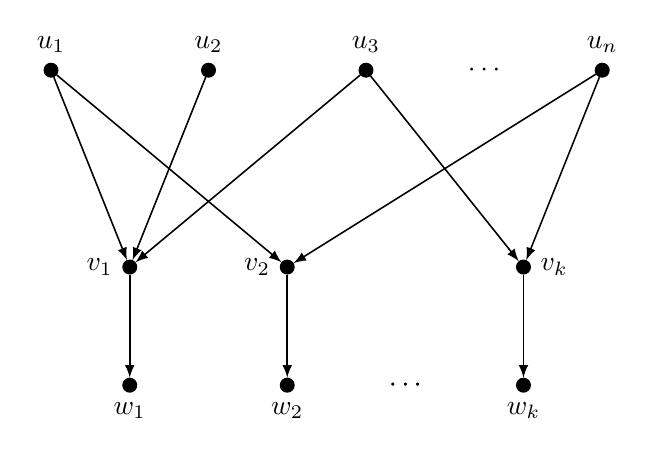
\begin{tikzpicture}
    \tikzstyle{vertex}=[draw, circle, fill=black, inner sep=0pt, minimum size=5pt]

    \node[vertex, label=above:$u_1$] (u1) at (0, 0) {};
    \node[vertex, label=above:$u_2$] (u2) at (2, 0) {};
    \node[vertex, label=above:$u_3$] (u3) at (4, 0) {};
    \node at (5.5, 0) {$\cdots$};
    \node[vertex, label=above:$u_n$] (un) at (7, 0) {};

    \node[vertex, label=left:$v_1$] (v1) at (1, -2.5) {};
    \node[vertex, label=left:$v_2$] (v2) at (3, -2.5) {};
    \node[] (ss) at (4.5, -4) {$\cdots$};
    \node[vertex, label=right:$v_k$] (vm) at (6, -2.5) {};

    \node[vertex, label=below:$w_1$] (w1) at (1, -4) {};
    \node[vertex, label=below:$w_2$] (w2) at (3, -4) {};
    \node[] (ss) at (4.5, -4) {$\cdots$};
    \node[vertex, label=below:$w_k$] (wm) at (6, -4) {};

    \draw[-latex,line width=0.2mm] (u1) to (v1);
    \draw[-latex,line width=0.2mm] (u2) to (v1);
    \draw[-latex,line width=0.2mm] (u3) to (v1);
    \draw[-latex,line width=0.2mm] (u1) to (v2);
    \draw[-latex,line width=0.2mm] (un) to (v2);
    \draw[-latex,line width=0.2mm] (u3) to (vm);
    \draw[-latex,line width=0.2mm] (un) to (vm);

    \draw[-latex,line width=0.2mm] (v1) to (w1);
    \draw[-latex,line width=0.2mm] (v2) to (w2);
    \draw[-latex,line width=0.2mm] (vm) to (wm);
\end{tikzpicture}
\caption{Gadget used in the proof of
Theorem~\ref{thm:hardness}. We reduce from a set cover
instance with $U = \{1, 2, \dots, n\}$ and subsets
$S_1 = \{1, 2, 3\}, S_2 = \{u_1, u_n\}, \dots,
S_k = \{u_3, u_n\}$.}
\end{figure}


\textsc{Corollary~\ref{cor:quantile}.}
\emph{
Let $(\alpha, W, s)$ be a
network of generalized FJ  dynamics,
let $k$ be a budget and $0 < q < 1$
be any quantile.
The problem to maximize the $q$-th
quantile of $x^\star(\alpha', W, s)$
subject to $\|\alpha' - \alpha\|_0 \le k$
cannot be approximated
to any multiplicative factor
unless $\mathsf{P} = \mathsf{NP}$.
}

\begin{proof}
This follows through a simple adaption
of the proof of Theorem~\ref{thm:hardness}.
Specifically, we can change the point
where the $q$-th quantile becomes positive
by modifying the number of isolated vertices to
$\ell=\lfloor (\frac 1 q - 1) n + (\frac 1 q - 2) m + \frac 1 q k \rfloor$.
This ensures
that the $q$-th percentile is $>0$
if and only if there exists a set cover.
\end{proof}
